\section{Analysis II: Drive-Cycle Efficiency}\label{sec:cycles}
The second analysis answers the question \emph{which drive uses less energy over a duty cycle?} It reuses the models of \cref{sec:models} unchanged, but instead of a fixed grid the operating points come from a time series, and the SOC and the temperatures evolve along it. It is implemented in \code{cycles.py} (cycle to machine profile) and \code{cycle_eval.py} (evaluation).

\subsection{From duty cycle to machine profile}\label{sec:profile}
Five kinds of cycle are supported. Each one returns the time $t$, the sample duration $\Delta t$, the machine speed $\omega_\mathrm{m}$ and the requested torque $T^*$ (\code{cycles.machine_profile}). \Cref{fig:profiles} shows the speed profiles.

\paragraph{Road-load model (car, bus, truck, train).} For a vehicle speed $v$ [\si{\metre\per\second}], acceleration $a$ and road slope $\alpha$, the tractive force at the wheel is (\code{applications.road_load_force})
\begin{equation}
F=k_\mathrm{m}\,m\,a+R(v,\alpha)+m\,g\sin\alpha,
\label{eq:roadload}
\end{equation}
with the rotating-mass factor $k_\mathrm{m}$; $R$ and the grade term are set to zero at standstill ($v\le\SI{0.01}{\metre\per\second}$), and
\begin{equation}
R=\begin{cases}\tfrac12\rho\,C_\mathrm{d}A\,v^2+\big(c_\mathrm{rr}+c_{\mathrm{rr},v}v\big)\,m\,g\cos\alpha & \text{road vehicles},\\[2pt] A_0+B_0v_\mathrm{kmh}+C_0v_\mathrm{kmh}^2 & \text{train (Davis)},\end{cases}\qquad R=0\ \text{if}\ v\le\SI{0.01}{\metre\per\second}.
\label{eq:resistance}
\end{equation}
With the wheel radius $r_\mathrm{w}$, gear ratio $G$ and gear efficiency $\eta_\mathrm{g}$, the machine speed and torque are (\code{cycles._wheel_to_machine})
\begin{equation}
\omega_\mathrm{m}=\frac{G\,v}{r_\mathrm{w}},\qquad
T^*=\begin{cases}\dfrac{F\,r_\mathrm{w}}{G\,\eta_\mathrm{g}} & F\ge0\ \text{(motoring)},\\[6pt] \dfrac{F\,r_\mathrm{w}\,\eta_\mathrm{g}}{G} & F<0\ \text{(regeneration)}.\end{cases}
\label{eq:wheel2machine}
\end{equation}
Gear losses are thus charged to the machine torque and are not part of the converter efficiency. \Cref{tab:vehicles} lists the vehicle data. Unless a gear ratio is given, it maps the top speed $v_\mathrm{top}$ to \SI{95}{\percent} of the maximum machine speed, $G=0.95\,\omega_\mathrm{m,max}r_\mathrm{w}/v_\mathrm{top}$ (\code{applications.gear_ratio}).

\begin{table}[ht]
\centering
\caption{Vehicle data of the road and rail applications ($m$ vehicle mass, $k_\mathrm{m}$ rotating-mass factor, $C_\mathrm{d}A$ drag area, $c_\mathrm{rr}$ rolling resistance, $r_\mathrm{w}$ wheel radius, $\eta_\mathrm{g}$ gear efficiency, $G$ gear ratio). The train uses the Davis coefficients $A_0=\SI{1000}{\newton}$, $B_0=\SI{10}{\newton\per(\kilo\metre\per\hour)}$, $C_0=\SI{0.10}{\newton\per(\kilo\metre\per\hour)\squared}$. The truck also has a speed-dependent rolling resistance $c_{\mathrm{rr},v}$ from the data file. Values are typical literature values (assumptions).}
\label{tab:vehicles}
\footnotesize
\begin{tabular}{@{}lrrrrrrr@{}}
\toprule
Application & $m$ [t] & $k_\mathrm{m}$ & $C_\mathrm{d}A$ [m$^2$] & $c_\mathrm{rr}$ & $r_\mathrm{w}$ [m] & $\eta_\mathrm{g}$ & $G$ \\
\midrule
Passenger car & 1.9 & 1.05 & 0.62 & 0.0085 & 0.33 & 0.97 & 8.4 \\
City bus & 15.0 & 1.08 & 5.00 & 0.007 & 0.48 & 0.96 & 19.0 \\
Heavy-duty truck & 40.0 & 1.00 & 5.00 & 0.006 & 0.50 & 0.96 & 10.6 \\
Off-road machine & \multicolumn{7}{c}{normalised / mode-based cycle, no vehicle model} \\
Marine vessel & \multicolumn{7}{c}{normalised / mode-based cycle, no vehicle model} \\
Regional train & 60.0 & 1.08 & Davis & -- & 0.43 & 0.97 & 5.6
\\
\bottomrule
\end{tabular}
\end{table}

\begin{figure}[ht]
\centering
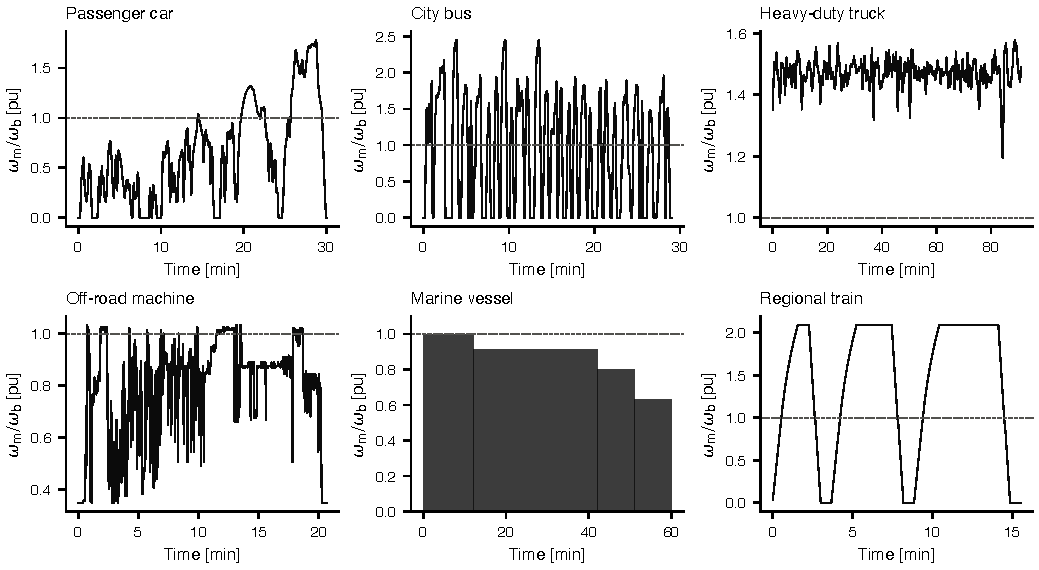
\includegraphics[width=\linewidth]{figures/paper_profiles.pdf}
\caption{Machine speed in per unit of base speed for the six duty cycles (dashed: base speed). Speed above 1 pu is field weakening.}
\label{fig:profiles}
\end{figure}

\paragraph{Speed cycles (car, bus).} The public speed traces WLTC Class~3b \cite{gtr15} and Braunschweig \cite{drivecat} (1~Hz, \code{data/cycles/}) give $v(t)$; the acceleration is the numerical gradient, $a=\mathrm{d}v/\mathrm{d}t$ (central differences), and \cref{eq:roadload,eq:wheel2machine} follow. The WHVC \cite{gtr4} is also in the data folder but is not used for the six presets.

\paragraph{Road cycle (truck).} The truck follows a measured road (distance and slope profile of the Södertälje--Norrköping route, \SI{119}{\kilo\metre}, from \code{so_no/}) under a proportional cruise controller. The longitudinal dynamics
\begin{equation}
\dot x=v,\qquad k_\mathrm{m}m\,\dot v=F_\mathrm{ctrl}-R\big(v,\alpha(x)\big)-mg\sin\alpha(x),\qquad
F_\mathrm{ctrl}=\operatorname{clip}\big(k_\mathrm{p}(v_\mathrm{set}-v),\pm F_\mathrm{max}\big)
\label{eq:cruise}
\end{equation}
are integrated with \code{scipy.integrate.solve_ivp} (RK45, output every \SI{1}{\second}) from $v_0=\SI{20}{\metre\per\second}$ until the end of the road, with $v_\mathrm{set}=\SI{80}{\kilo\metre\per\hour}$, $k_\mathrm{p}=\SI{e4}{\newton\per(\metre\per\second)}$ and $F_\mathrm{max}=\SI{7000}{\newton\metre}/r_\mathrm{w}$. Then $a$ is the gradient of $v(t)$, and \cref{eq:roadload,eq:wheel2machine} give the machine profile.

\paragraph{Normalised cycle (off-road machine).} The NRTC \cite{eu2017_654} gives speed in percent between idle and rated speed, and torque in percent of the maximum torque at that speed. With rated speed $\omega_\mathrm{r}=\omega_\mathrm{b}$ and idle speed $\omega_\mathrm{i}=0.35\,\omega_\mathrm{r}$,
\begin{equation}
\omega_\mathrm{m}=\omega_\mathrm{i}+\frac{n_\%}{100}(\omega_\mathrm{r}-\omega_\mathrm{i}),\qquad T^*=\frac{T_\%}{100}\min\Big(T_\mathrm{b},\frac{P_\mathrm{b}}{\omega_\mathrm{m}}\Big).
\label{eq:nrtc}
\end{equation}
The NRTC table contains no motoring (drag) points (see the README of \code{data/cycles/}); the code would treat such points as zero torque.

\paragraph{Mode cycle (marine vessel).} The ISO~8178 E3 propeller-law cycle \cite{iso8178_4} has four steady modes with speed $n_i=(1.00,0.91,0.80,0.63)$ pu, power $p_i=(1.00,0.75,0.50,0.25)$ pu and time weight $w_i=(0.20,0.50,0.15,0.15)$. With rated speed $\omega_\mathrm{b}$ and continuous rating $0.9P_\mathrm{b}$, mode $i$ lasts $w_i\cdot\SI{3600}{\second}$ at $\omega_{\mathrm{m},i}=n_i\omega_\mathrm{b}$ and $T_i^*=0.9\,p_iP_\mathrm{b}/\omega_{\mathrm{m},i}$.

\paragraph{Synthetic rail cycle (regional train).} A regional run with three station-to-station sections (\SIlist{4;7;10}{\kilo\metre}), a line speed of \SI{120}{\kilo\metre\per\hour}, maximum acceleration and deceleration of \SI{0.8}{\metre\per\second\squared} and \SI{40}{\second} dwell is generated with a time step of \SI{1}{\second} (\code{cycles.rail_cycle}). In each step the train brakes if the remaining distance is not larger than the braking distance $v^2/(2a_\mathrm{dec})$; otherwise it accelerates with
\begin{equation}
a=\min\Big(a_\mathrm{max},\ \frac{\min\big(F_\mathrm{lim},\,P_\mathrm{lim}/\max(v,0.1)\big)-R(v)}{k_\mathrm{m}m}\Big),\quad P_\mathrm{lim}=0.9P_\mathrm{b}\eta_\mathrm{g},\ \ F_\mathrm{lim}=\frac{0.9\,T_\mathrm{b}G\eta_\mathrm{g}}{r_\mathrm{w}},
\label{eq:rail}
\end{equation}
up to the line speed, and then cruises. Then \cref{eq:roadload,eq:wheel2machine} apply.

\subsection{Sample-by-sample evaluation}\label{sec:eval}
\Cref{alg:cycle} gives the algorithm of \code{cycle_eval.evaluate_cycle}. For each sample, the cell state, the voltage limits, the torque that both drives can deliver, the losses of both drives and the new SOC are computed.

\begin{lstlisting}[caption={Cycle evaluation (\code{cycle_eval.evaluate_cycle}) from initial SOC $z_0$.}, label={alg:cycle}]
d $\leftarrow$ design(p);  (t, $\Delta t$, $\omega_\mathrm{m}$, T*) $\leftarrow$ machine_profile(app);  $\omega_\mathrm{m}$ $\leftarrow$ clip($\omega_\mathrm{m}$, 0, $\omega_\mathrm{m,max}$)
z$_X$ $\leftarrow$ z$_0$ for X in {2L, BI};  n$_\mathrm{cells}^X$ $\leftarrow$ cells of each pack
for each sample k with ($\omega_\mathrm{m}$, T*, $\Delta t$):
    cell$_X$ $\leftarrow$ cell_state(p, z$_X$)
    if T* = 0 and $\omega_\mathrm{m}$ = 0: T $\leftarrow$ 0, all losses 0, temperatures = ambient, converter off
    else:
        $\hat v^X_\mathrm{max}$ $\leftarrow$ Eq. $\eqref{eq:vmax}$ with the OCV of cell$_X$
        T$_\mathrm{lim}$ $\leftarrow$ P$_\mathrm{b}$/$\omega_\mathrm{m}$ (1 - 10$^{-9}$);   T$_\mathrm{cmd}$ $\leftarrow$ clip(T*, -T$_\mathrm{lim}$, T$_\mathrm{lim}$)
        for X in {2L, BI}: (T$_X$, i$_X$) $\leftarrow$ feasible_torque(T$_\mathrm{cmd}$, $\hat v^X_\mathrm{max}$)       // Eq. $\eqref{eq:bisect}$
        T $\leftarrow$ sign(T$_\mathrm{cmd}$) min(|T$_\mathrm{2L}$|, |T$_\mathrm{BI}$|)                                // common torque
        for X with |T$_X$| $\neq$ |T|: i$_X$ $\leftarrow$ MTPA at the common torque T
        if some i$_X$ is None: mark sample infeasible, losses 0, T$_\mathrm{j}$ = T$_\mathrm{c}$ = NaN
        else: (P$_\mathrm{c}$, P$_\mathrm{s}$, P$_\mathrm{b}$, T$_\mathrm{j}$, T$_\mathrm{c}$)$_X$ $\leftarrow$ losses_2l / losses_bimmc
    P $\leftarrow$ $\omega_\mathrm{m}$ T;  T$_\mathrm{cell}^X$ $\leftarrow$ Eq. $\eqref{eq:tcell}$
    for X: I$_\mathrm{cell}^X$ $\leftarrow$ (P + P$_\mathrm{c}$ + P$_\mathrm{s}$ + P$_\mathrm{b}$) / (n$_\mathrm{cells}^X$ V$_\mathrm{cell}$);  z$_X$ $\leftarrow$ clip(z$_X$ - I$_\mathrm{cell}^X$ $\Delta t$ / (3600 Q$_\mathrm{cell}$), 0, 1)
accumulate energies and metrics, Eqs. $\eqref{eq:energies}$-$\eqref{eq:etacyc}$
\end{lstlisting}

\paragraph{Speed clipping and standstill.} The speed is limited to the range $[0,\omega_\mathrm{m,max}]$ (regeneration is represented by negative torque only). At standstill with zero torque the converters are off.

\paragraph{Common torque.} Both drives must deliver the same mechanical cycle, so that their efficiencies are comparable. The commanded torque is first limited by the rated power, $|T_\mathrm{cmd}|\le P_\mathrm{b}/\omega_\mathrm{m}$. If \cref{eq:mtpa} is infeasible at $T_\mathrm{cmd}$ for one of the drives (voltage or current limit), \code{feasible_torque} bisects the interval $[0,T_\mathrm{cmd}]$ ten times,
\begin{equation}
\text{keep the largest feasible } T\in[0,T_\mathrm{cmd}]\ \text{found by}\ T_{j+1}=\tfrac12(T_j^\mathrm{lo}+T_j^\mathrm{hi}),\ j=1\dots10,
\label{eq:bisect}
\end{equation}
which resolves the torque to $|T_\mathrm{cmd}|/2^{10}$. The delivered torque is the \emph{smaller} of the two drives' feasible torques, so neither drive gets an unfair advantage. The remainder, $T^*-T$, is assumed to be taken by the mechanical brake (regeneration) or not delivered (motoring) and is reported as ``clipped'' energy.

\paragraph{BI-MMC speed floor.} The time-domain battery simulation needs an electrical period and a stable step (\cref{sec:lossbimmc}). For low speeds, the BI-MMC loss is therefore evaluated at the effective speed $\omega_\mathrm{m,eff}=\max\big(\omega_\mathrm{m},\,2\pi f_\mathrm{c,min}/(m_\mathrm{f}p)\big)$ with $f_\mathrm{c,min}=\SI{50}{\hertz}$ (i.e.\ $f_\mathrm{e}\ge\SI{25}{\hertz}$ for $m_\mathrm{f}=2$), for the voltages, the carrier frequency (and hence switching and battery loss) and the gating, while the currents and the torque are those of the actual operating point. This floor makes the BI-MMC loss at creep speed an estimate, not an exact value.

\paragraph{State of charge.} Each pack is a power source at its OCV. The power drawn from it is the mechanical power plus the total loss (the cell resistance loss is part of $P_\mathrm{b}$), shared equally by the $n_\mathrm{cells}$ cells ($N_\mathrm{s}N_\mathrm{p}$ for the 2L pack, $3\Nsm\Nssm\Npsm$ for the BI-MMC):
\begin{equation}
I_\mathrm{cell}=\frac{P+P_\mathrm{c}+P_\mathrm{s}+P_\mathrm{b}}{n_\mathrm{cells}V_\mathrm{cell}(z_k)},\qquad
z_{k+1}=\operatorname{clip}\Big(z_k-\frac{I_\mathrm{cell}\Delta t}{3600\,Q_\mathrm{cell}},\,0,\,1\Big).
\label{eq:soc}
\end{equation}
The two drives therefore follow slightly different SOC trajectories, and the voltage limit and the cell parameters are updated at every step.

\paragraph{Thermal state.} Junction, case and cell temperatures are the \emph{steady-state} values of \cref{eq:thermal2l,eq:tcell} for the loss of the present sample. There is no thermal capacitance, so the peak temperatures are upper bounds for samples shorter than the thermal time constants.

\subsection{Cycle metrics}\label{sec:metrics}
With $P_k=\omega_{\mathrm{m},k}T_k$ and the sample duration $\Delta t_k$, the energies are ($\lfloor x\rfloor^+=\max(x,0)$)
\begin{align}
E_\mathrm{mot}&=\sum_k\lfloor P_k\rfloor^+\Delta t_k, & E_\mathrm{reg}&=\sum_k\lfloor -P_k\rfloor^+\Delta t_k, \label{eq:energies}\\
E_x^X&=\sum_kP_{x,k}^X\Delta t_k\quad(x\in\{\mathrm{c},\mathrm{s},\mathrm{b}\}),& E_\mathrm{loss}^X&=E_\mathrm{c}^X+E_\mathrm{s}^X+E_\mathrm{b}^X. \label{eq:eloss}
\end{align}
The cycle efficiency charges the losses to the traction energy throughput, and the difference between the drives is given in percentage points (pp):
\begin{equation}
\etacyc^X=1-\frac{E_\mathrm{loss}^X}{E_\mathrm{mot}+E_\mathrm{reg}},\qquad
\Delta\etacyc=\etacyc^\mathrm{BI}-\etacyc^\mathrm{2L}.
\label{eq:etacyc}
\end{equation}
Further outputs are the net battery energy $E_\mathrm{mot}-E_\mathrm{reg}+E_\mathrm{loss}$ (per \SI{100}{\kilo\metre} for vehicle cycles), the relative loss change $E_\mathrm{loss}^\mathrm{BI}/E_\mathrm{loss}^\mathrm{2L}-1$, the final SOC, the peak temperatures, the clipped energies in motoring and regeneration, $\sum\big(\lfloor P^*\rfloor^+-\lfloor P\rfloor^+\big)\Delta t$ and $\sum\big(\lfloor -P^*\rfloor^+-\lfloor -P\rfloor^+\big)\Delta t$ with $P^*=\omega_\mathrm{m}T^*$, and the share of mechanical energy delivered below base speed,
\begin{equation}
\sigma_\mathrm{b}=\frac{\sum_k|P_k|\Delta t_k\,[\omega_{\mathrm{m},k}\le\omega_\mathrm{b}]}{\sum_k|P_k|\Delta t_k},
\label{eq:share}
\end{equation}
which will turn out to be the best predictor of $\Delta\etacyc$ (\cref{sec:results}). \Cref{eq:etacyc} differs from the point efficiency \cref{eq:eta}: it weights each operating point by the energy processed there, which is what a drive cycle requires.

\paragraph{Relation to the maps.} \Cref{eq:etacyc} is the energy-weighted mean of the loss maps along the cycle, apart from three effects that the maps do not have: the SOC changes along the cycle, the common torque is limited by the weaker drive, and the BI-MMC speed floor. The cycle evaluation therefore does not interpolate the maps. The map backgrounds in \cref{sec:results} are used only to visualise where the cycle energy lies.
